\hypertarget{mr.-potato-head}{%
\section{Mr.~Potato Head}\label{mr.-potato-head}}

\begin{figure}[!ht]
  \begin{adjustwidth}{-\oddsidemargin-1in}{-\rightmargin}
    \centering
    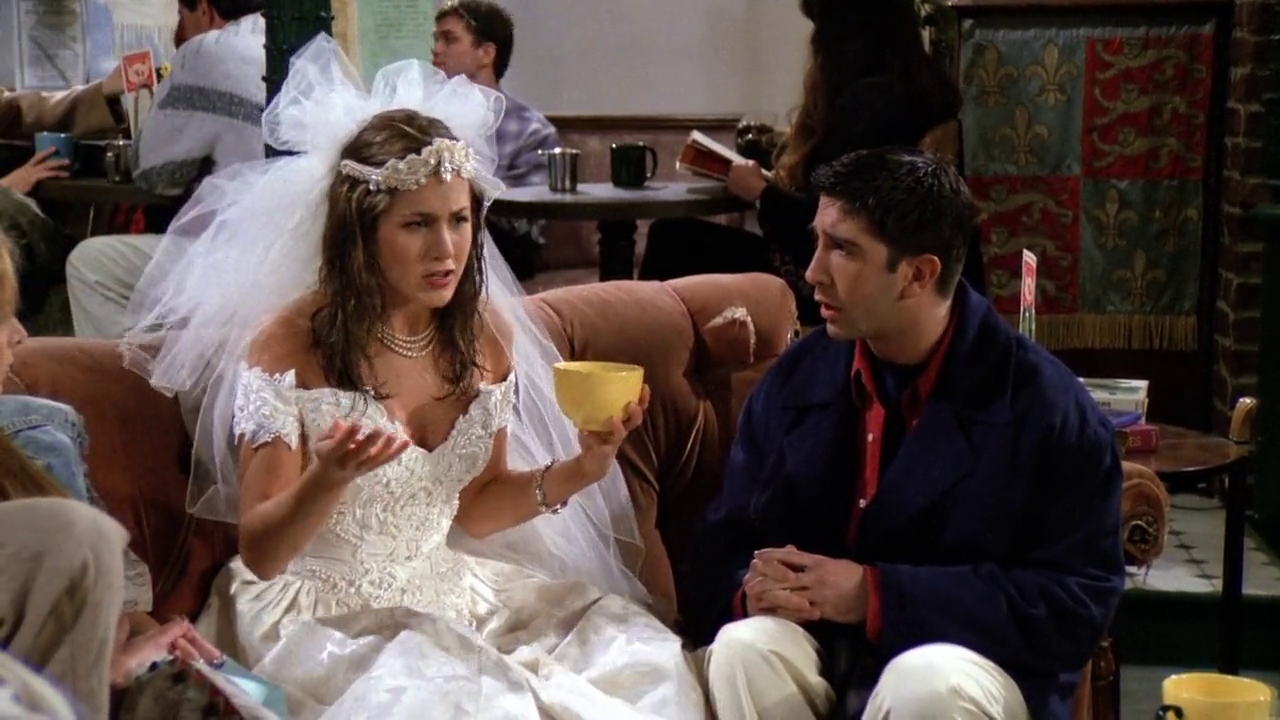
\includegraphics[trim={0 5cm 0 2cm,}, clip, width=\paperwidth]{./S01/img/1/mr-potato-head.png}
    \caption{Mr. Potato Head\label{fig:mr-potato-head}}
  \end{adjustwidth}
\end{figure}

\begin{tcolorbox}[enhanced,center upper,
    drop fuzzy shadow southeast, boxrule=0.3pt,
    lower separated=false,
    colframe=black!30!dialogoBorder,colback=white]
\begin{minipage}[c]{0.14\linewidth}
  \raisebox{\dimexpr-\height+\ht\strutbox\relax}{
    
\includegraphics[width=1.5cm]{./assets/img/rachel.png}
  }
   & \centering \scriptsize{Rachel}
\end{minipage}
\hspace{.1mm}
\begin{minipage}[c]{0.8\linewidth}
  \textbf{- [...] and that's when it hit me: How much Barry looks like Mr. Potato Head.}\\
  - [...] e me dei conta: O quanto Barry se parece com o Mr. Potato Head.
\end{minipage}
\end{tcolorbox}

\saveparinfos
\noindent
\begin{minipage}[c]{0.5\textwidth}\useparinfo

Rachel menciona que Barry, seu ex-noivo, parece com o \emph{Mr.~Potato
Head.} Trata-se de um brinquedo inventado por George Lerner, lançado
pela Hasbro em 1952. Em sua versão original havia apenas as partes, tais
como: os olhos, as orelhas e a boca, e era obrigação dos pais fornecerem
uma batata de verdade para formar a cabeça.

O \emph{Mr.~Potato Head} também pode ser visto nos filmes de \emph{Toy
Story} (1995, 1999, 2010, 2019), como um dos brinquedos do Andy.

\end{minipage}\hfill
\begin{minipage}[c]{0.45\textwidth}

\begin{figure}
  \centering
  \begin{tikzpicture}
    \node [inner sep=0pt] at (0,0) {
      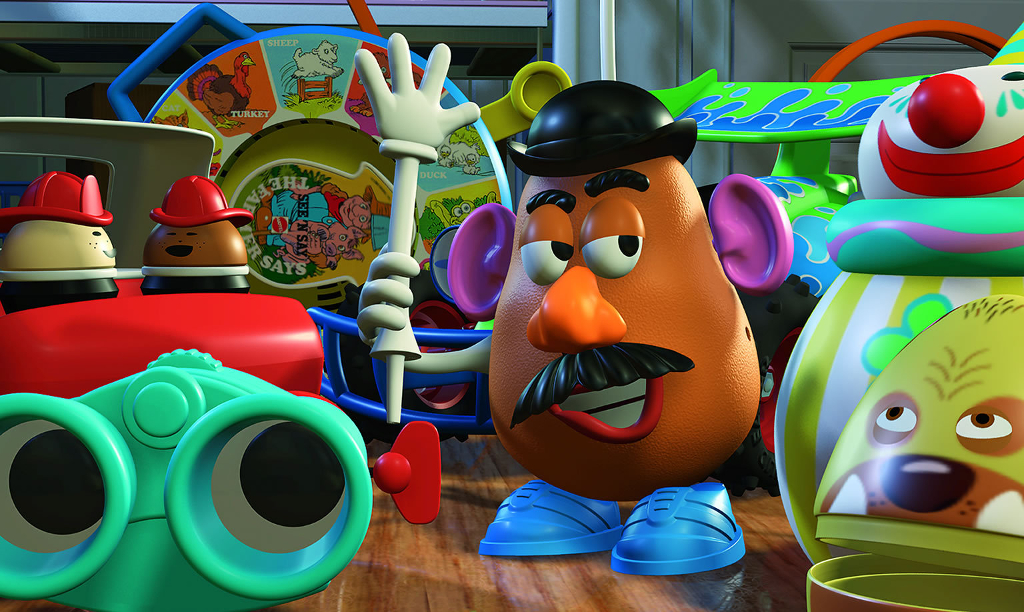
\includegraphics[width=0.8\textwidth,keepaspectratio]{./S01/img/1/mr-potato-head-toy-story.jpg}
    };
    \draw [white, rounded corners=\ClipSep, line width=\ClipSep]
    (current bounding box.north west) --
    (current bounding box.north east) --
    (current bounding box.south east) --
    (current bounding box.south west) -- cycle
    ;
    \end{tikzpicture}
    \caption{Mr. Potato Head (Toy Story)\label{fig:mr-potato-head-toy-story}}
\end{figure}

\end{minipage}

\hypertarget{referuxeancias}{%
\subsection{Referências}\label{referuxeancias}}

\begin{itemize}
\tightlist
\item
  \sloppy V&A Museum of Childhood. \url{https://www.vam.ac.uk/moc/collections/mr-potato-head/}
\item
  \sloppy Toy Story (IMDB). \url{https://www.imdb.com/title/tt0114709/}
\end{itemize}

\hypertarget{tres-destinos}{%
\section{Tres Destinos}\label{tres-destinos}}

\begin{figure}[!ht]
  \begin{adjustwidth}{-\oddsidemargin-1in}{-\rightmargin}
    \centering
    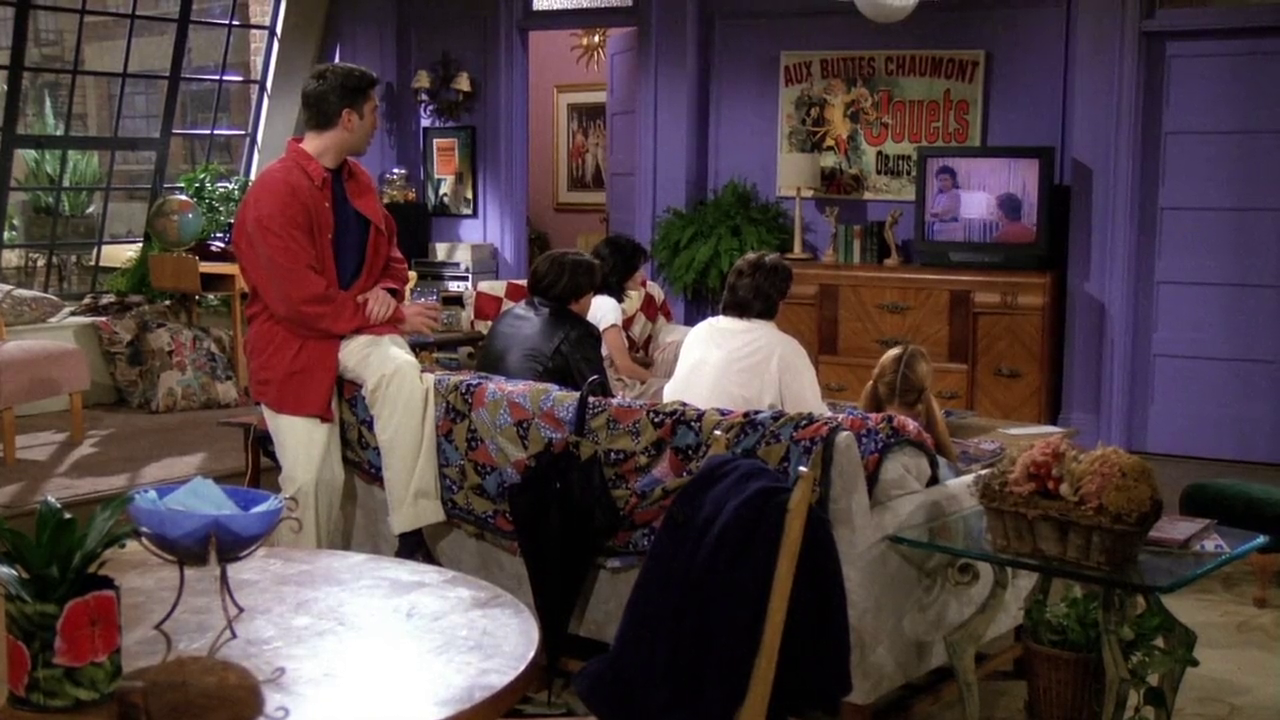
\includegraphics[trim={0 7cm 0 1.5cm,}, clip, width=\paperwidth]{./S01/img/1/tres-destinos.png}
    \caption{Tres Destinos\label{fig:tres-destinos}}
  \end{adjustwidth}
\end{figure}

Os amigos são vistos assistindo a telenovela \emph{Tres Destinos}
(1993), produzida para o mercado hispânico nos Estados Unidos. É a
clássica novela mexicana, do tipo popularmente exibida no Brasil, que
conta a história de 3 jovens irmãs unidas e separadas pelo mesmo homem,
com todos os ingredientes usuais: intriga, paixão, vingança, ódio,
ternura e amor.

\hypertarget{referuxeancias-1}{%
\subsection{Referências}\label{referuxeancias-1}}

\begin{itemize}
\tightlist
\item
  \sloppy EcuRed. \url{https://www.ecured.cu/Tres_destinos_(Telenovela)}
\item
  \sloppy IMDB. \url{https://www.imdb.com/title/tt0211876/}
\item
  \sloppy Abertura (YouTube). \url{https://www.youtube.com/watch?v=kfIk131FZxU}
\end{itemize}

\hypertarget{my-favorite-things}{%
\section{My Favorite Things}\label{my-favorite-things}}

\begin{figure}[!ht]
  \begin{adjustwidth}{-\oddsidemargin-1in}{-\rightmargin}
    \centering
    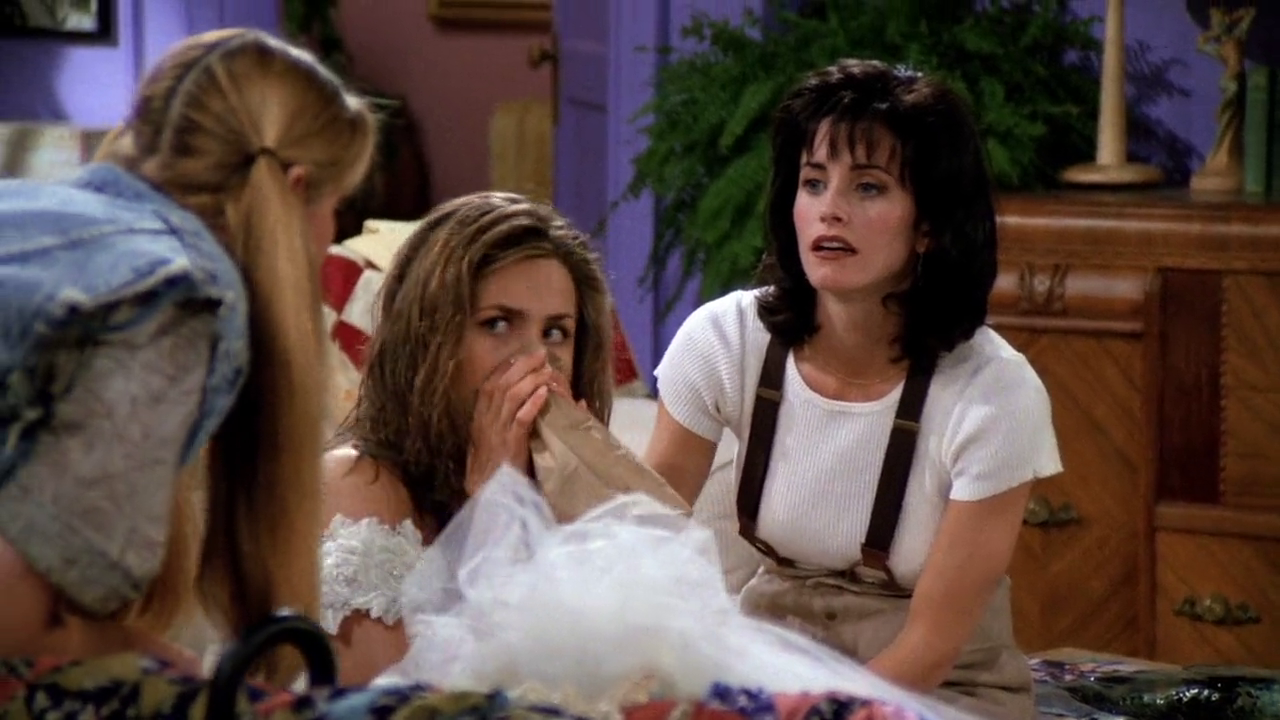
\includegraphics[trim={0 6cm 0 0.5cm,}, clip, width=\paperwidth]{./S01/img/1/my-favorite-things.png}
    \caption{My Favorite Things\label{fig:my-favorite-things}}
  \end{adjustwidth}
\end{figure}

Para acalmar Rachel, Phoebe canta uma versão própria da música \emph{My
Favorite Things} do musical \emph{The Sound of Music} (1959). Em 1965
foi lançado o filme, conhecido no Brasil como \emph{A Noviça Rebelde.}

A música expressa que você deve lembrar de suas coisas favoritas sempre
que se sentir triste.

\bigskip
\begin{tcolorbox}[enhanced,
    drop fuzzy shadow southeast, boxrule=0.3pt,
    lower separated=false, sidebyside, sidebyside align=top,
    halign=flush right, halign lower=left,
    colframe=black!30!dialogoBorder,colback=musicaBg]
\includegraphics[width=0.4cm]{./assets/img/icon-music.png}\\
When I’m feeling sad\\I simply remember my favorite things\\
\tcblower
\includegraphics[width=0.4cm]{./assets/img/icon-language.png}\\
Quando me sinto triste\\Simplesmente lembro de minhas coisas favoritas\\
\end{tcolorbox}

\begin{center}\rule{0.5\linewidth}{0.5pt}\end{center}

Versão da Phoebe:

\bigskip
\begin{tcolorbox}[enhanced,
    drop fuzzy shadow southeast, boxrule=0.3pt,
    lower separated=false, sidebyside, sidebyside align=top,
    halign=flush right, halign lower=left,
    colframe=black!30!dialogoBorder,colback=musicaBg]
\includegraphics[width=0.4cm]{./assets/img/icon-music.png}\\
Raindrops on roses\\And whiskers on kittens\\Doorbells and sleigh bells\\And something with mittens\\La la la la something with strings\\
\tcblower
\includegraphics[width=0.4cm]{./assets/img/icon-language.png}\\
Pingos de chuva em rosas\\E bigodes de gatinhos\\Campainhas e sinos\\E algo com luvas de lã\\La la la la algo com cordas\\
\end{tcolorbox}

Versão original:

\bigskip
\begin{tcolorbox}[enhanced,
    drop fuzzy shadow southeast, boxrule=0.3pt,
    lower separated=false, sidebyside, sidebyside align=top,
    halign=flush right, halign lower=left,
    colframe=black!30!dialogoBorder,colback=musicaBg]
\includegraphics[width=0.4cm]{./assets/img/icon-music.png}\\
Raindrops on roses\\And whiskers on kittens\\Bright copper kettles\\And warm woolen mittens\\Brown paper packages\\Tied up with strings\\
\tcblower
\includegraphics[width=0.4cm]{./assets/img/icon-language.png}\\
Pingos de chuva em rosas\\E bigodes de gatinhos\\Brilhantes tachos de cobre\\E quentes luvas de lã\\Pacotes de papel pardo\\Amarrado com cordas\\
\end{tcolorbox}

\begin{tcolorbox}[enhanced,center upper,
    drop fuzzy shadow southeast, boxrule=0.3pt,
    lower separated=false,
    colframe=black!30!dialogoBorder,colback=white]
\begin{minipage}[c]{0.14\linewidth}
  \raisebox{\dimexpr-\height+\ht\strutbox\relax}{
    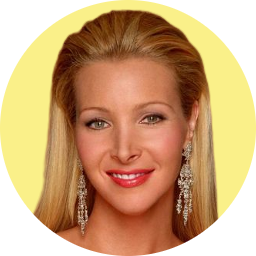
\includegraphics[width=1.5cm]{./assets/img/phoebe.png}
  }
   & \centering \scriptsize{Phoebe}
\end{minipage}
\hspace{.1mm}
\begin{minipage}[c]{0.8\linewidth}
  \textbf{- I helped.}\\
  - Eu ajudei.
\end{minipage}
\end{tcolorbox}

\hypertarget{referuxeancias-2}{%
\subsection{Referências}\label{referuxeancias-2}}

\begin{itemize}
\tightlist
\item
  \sloppy Trecho do filme The Sound of Music, em que é possível ouvir My Favorite Things (Youtube). \url{https://www.youtube.com/watch?v=DGABqdbtQnA}
\item
  \sloppy Wikipédia. \url{https://en.wikipedia.org/wiki/My_Favorite_Things_(song)}
\item
  \sloppy A Noviça Rebelde (IMDB). \url{https://www.imdb.com/title/tt0059742/}
\item
  \sloppy Letra e tradução - Vagalume. \url{https://www.vagalume.com.br/julie-andrews/my-favorite-things-traducao.html}
\end{itemize}

\hypertarget{maina-la-voyante}{%
\section{Maina La Voyante}\label{maina-la-voyante}}

\begin{figure}[!ht]
  \begin{adjustwidth}{-\oddsidemargin-1in}{-\rightmargin}
    \centering
    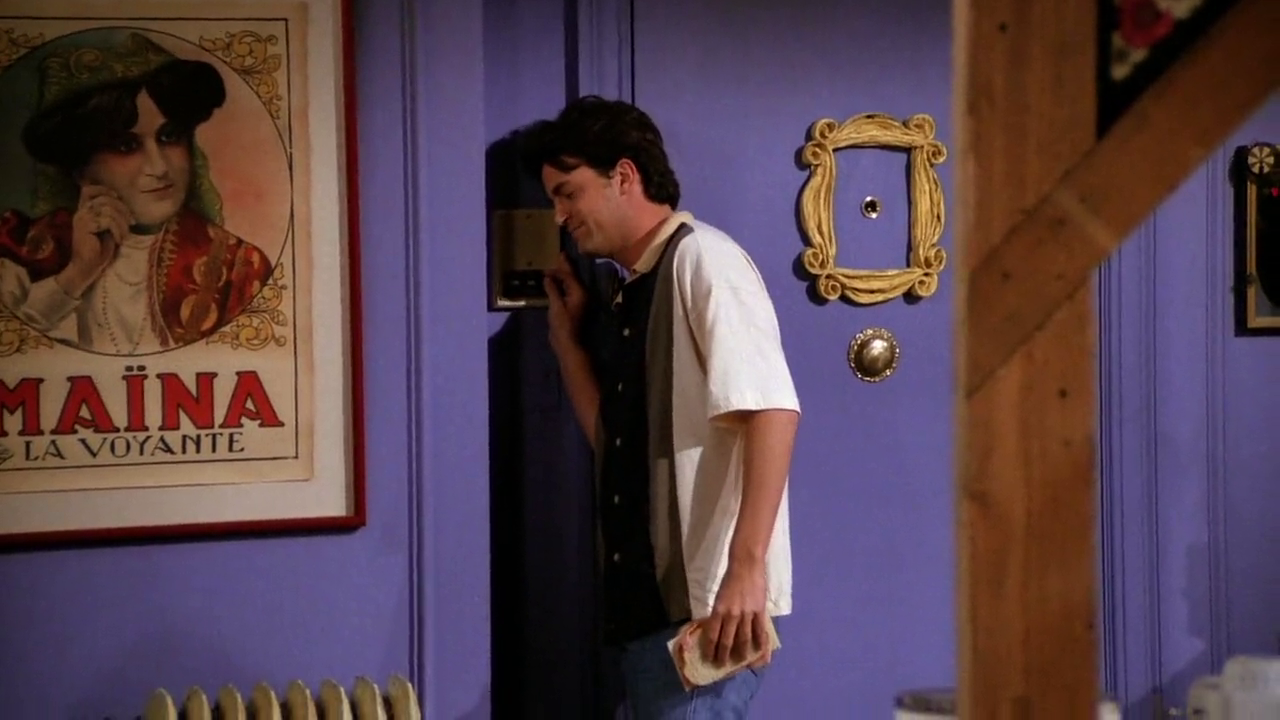
\includegraphics[trim={0 8cm 0 0.5cm,}, clip, width=\paperwidth]{./S01/img/1/maina-la-voyante.png}
    \caption{Maina La Voyante\label{fig:maina-la-voyante}}
  \end{adjustwidth}
\end{figure}

\saveparinfos
\noindent
\begin{minipage}[c]{0.5\textwidth}\useparinfo

Quando Chandler vai atender ao interfone, o poster \emph{Maina La
Voyante} pode ser visto, obra do ilustrador francês Louis Galice
(1864-1935).

\end{minipage}\hfill
\begin{minipage}[c]{0.6\textwidth}

\begin{figure}
  \centering
  \begin{tikzpicture}
    \node [inner sep=0pt] at (0,0) {
      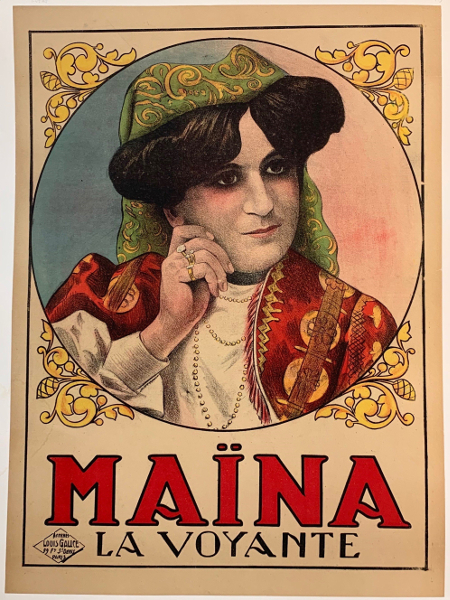
\includegraphics[width=0.6\textwidth,keepaspectratio]{./S01/img/1/maina-la-voyante-poster.jpg}
    };
    \draw [white, rounded corners=\ClipSep, line width=\ClipSep]
    (current bounding box.north west) --
    (current bounding box.north east) --
    (current bounding box.south east) --
    (current bounding box.south west) -- cycle
    ;
    \end{tikzpicture}
    \caption{Maina La Voyante - Poster\label{fig:maina-la-voyante-poster}}
\end{figure}

\end{minipage}

\hypertarget{referuxeancias-3}{%
\subsection{Referências}\label{referuxeancias-3}}

\begin{itemize}
\tightlist
\item
  \sloppy PosterMuseum. \url{https://postermuseum.com/products/maina-la-voyante}
\end{itemize}

\hypertarget{speed-racer}{%
\section{Speed Racer}\label{speed-racer}}

\begin{figure}[!ht]
  \begin{adjustwidth}{-\oddsidemargin-1in}{-\rightmargin}
    \centering
    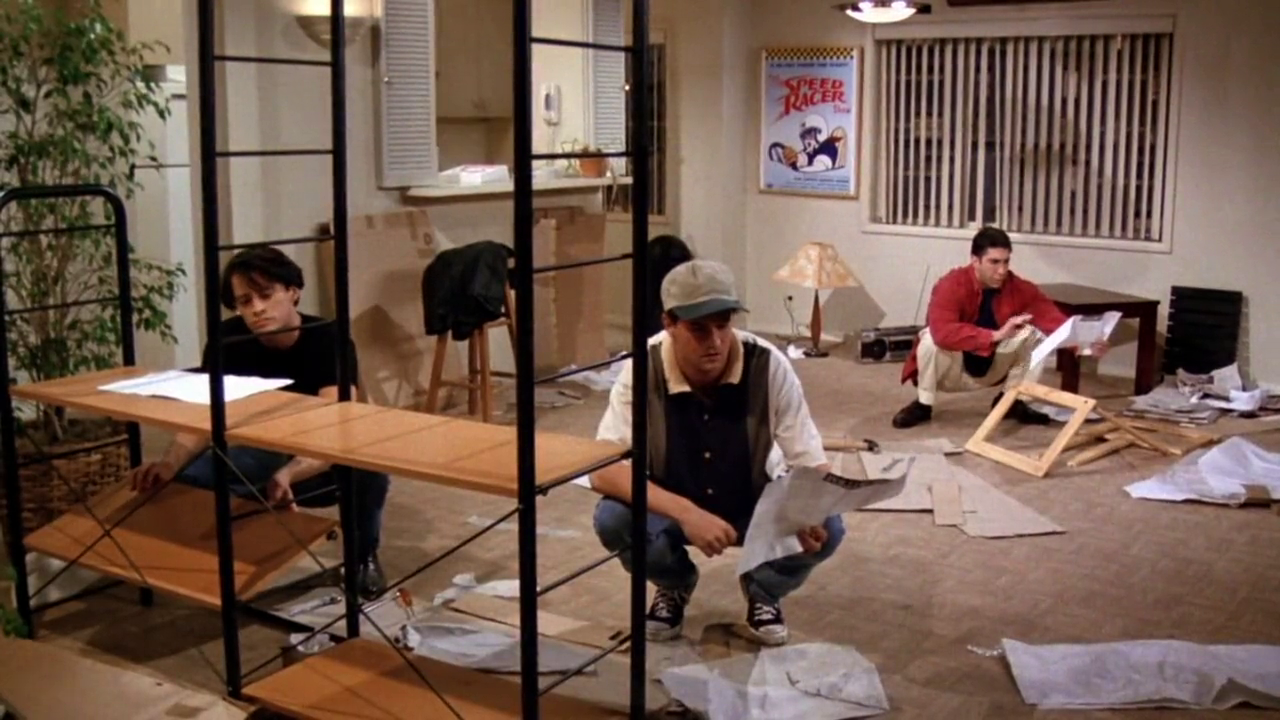
\includegraphics[trim={0 10cm 0 1cm,}, clip, width=\paperwidth]{./S01/img/1/speed-racer.png}
    \caption{Speed Racer\label{fig:speed-racer}}
  \end{adjustwidth}
\end{figure}

\saveparinfos
\noindent
\begin{minipage}[c]{0.5\textwidth}\useparinfo

No novo apartamento do Ross, é possível ver um poster de \emph{The Speed
Racer Show} (1967--1968) produzida pela \emph{Tatsunoko Production}.
Trata-se de uma série japonesa animada protagonizada por \emph{Go
Mifune}, conhecido como \emph{Speed Racer}. É baseada no mangá
\emph{Mach Go Go Go} (1966) criada por \emph{Tatsuo Yoshida}.

\end{minipage}\hfill
\begin{minipage}[c]{0.5\textwidth}

\begin{figure}
  \centering
  \begin{tikzpicture}
    \node [inner sep=0pt] at (0,0) {
      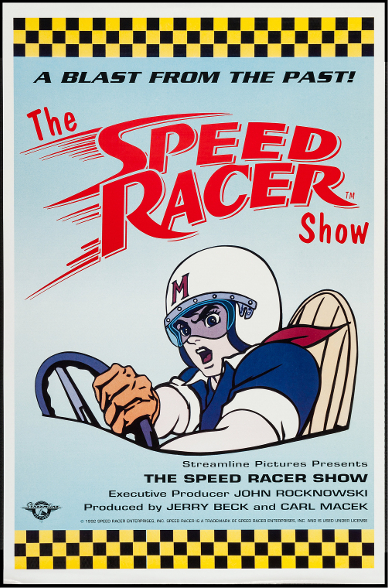
\includegraphics[width=0.8\textwidth,keepaspectratio]{./S01/img/1/speed-racer-poster.jpeg}
    };
    \draw [white, rounded corners=\ClipSep, line width=\ClipSep]
    (current bounding box.north west) --
    (current bounding box.north east) --
    (current bounding box.south east) --
    (current bounding box.south west) -- cycle
    ;
    \end{tikzpicture}
    \caption{Speed Racer poster\label{fig:speed-racer-poster}}
\end{figure}

\end{minipage}

\hypertarget{referuxeancias-4}{%
\subsection{Referências}\label{referuxeancias-4}}

\begin{itemize}
\tightlist
\item
  \sloppy IMDB. \url{https://www.imdb.com/title/tt0061300/}
\item
  \sloppy Review do Omelete. \url{https://www.omelete.com.br/series-tv/lembra-desse-speed-racer-a-serie-original}
\item
  \sloppy Abertura (YouTube). \url{https://www.youtube.com/watch?v=suCm1w_KTiY}
\end{itemize}

\hypertarget{joanie-loves-chachi}{%
\section{Joanie Loves Chachi}\label{joanie-loves-chachi}}

\begin{figure}[!ht]
  \begin{adjustwidth}{-\oddsidemargin-1in}{-\rightmargin}
    \centering
    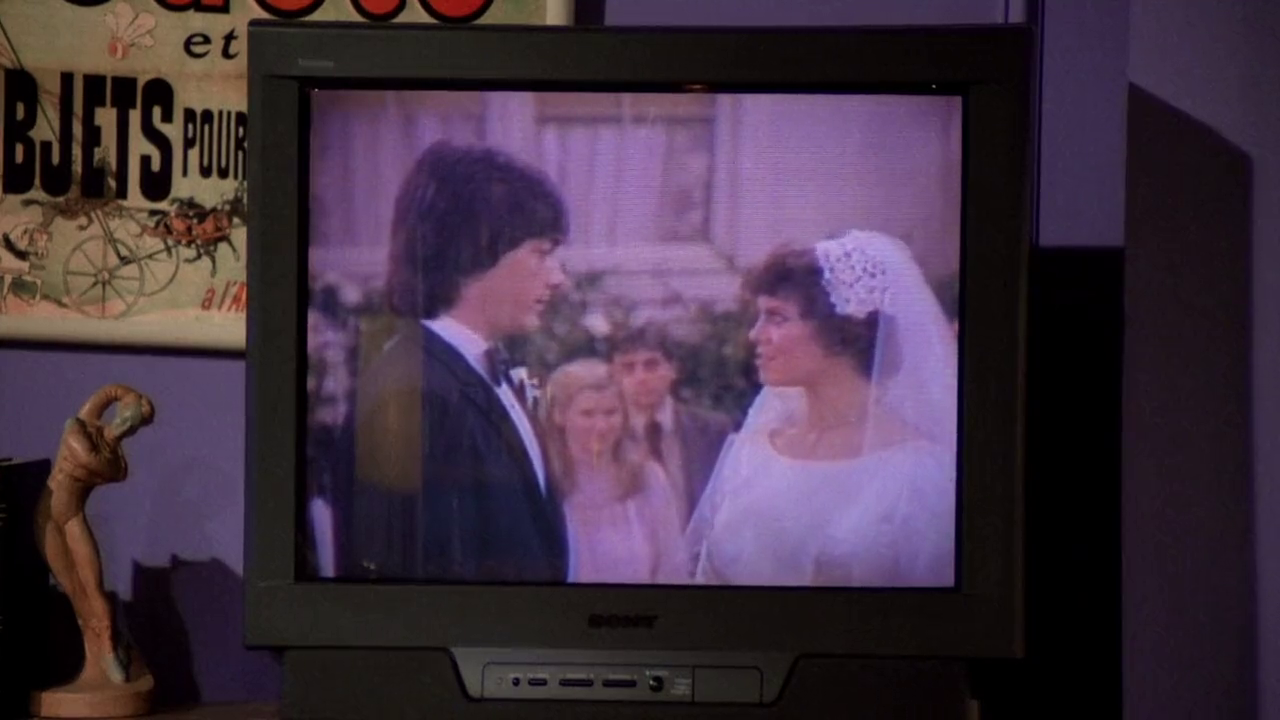
\includegraphics[trim={0 4cm 0 2cm,}, clip, width=\paperwidth]{./S01/img/1/joanie-loves-chachi.png}
    \caption{Joanie Loves Chachi\label{fig:joanie-loves-chachi}}
  \end{adjustwidth}
\end{figure}

\begin{tcolorbox}[enhanced,center upper,
    drop fuzzy shadow southeast, boxrule=0.3pt,
    lower separated=false,
    colframe=black!30!dialogoBorder,colback=white]
\begin{minipage}[c]{0.14\linewidth}
  \raisebox{\dimexpr-\height+\ht\strutbox\relax}{
    
\includegraphics[width=1.5cm]{./assets/img/rachel.png}
  }
   & \centering \scriptsize{Rachel}
\end{minipage}
\hspace{.1mm}
\begin{minipage}[c]{0.8\linewidth}
  \textbf{- But Joanie loved Chachi. That's the difference.}\\
  - Mas Joanie ama Chachi. Essa é a diferença.
\end{minipage}
\end{tcolorbox}

No apartamento de Monica, Rachel, ainda em seu vestido de noiva, assiste
a \emph{Joanie Loves Chachi} (1982--1983) - \emph{spin off} de
\emph{Happy Days} (1974) -, uma série de TV que mostra as aventuras
românticas de Joanie Cunningham e Chachi Arcola, buscando uma carreira
musical em Chicago.

\hypertarget{referuxeancias-5}{%
\subsection{Referências}\label{referuxeancias-5}}

\begin{itemize}
\tightlist
\item
  \sloppy IMDB. \url{https://www.imdb.com/title/tt0083433/}
\item
  \sloppy Wikipédia. \url{https://en.wikipedia.org/wiki/Joanie_Loves_Chachi}
\end{itemize}

\hypertarget{billy-dont-be-a-hero}{%
\section{Billy, don't be a hero}\label{billy-dont-be-a-hero}}

\begin{figure}[!ht]
  \begin{adjustwidth}{-\oddsidemargin-1in}{-\rightmargin}
    \centering
    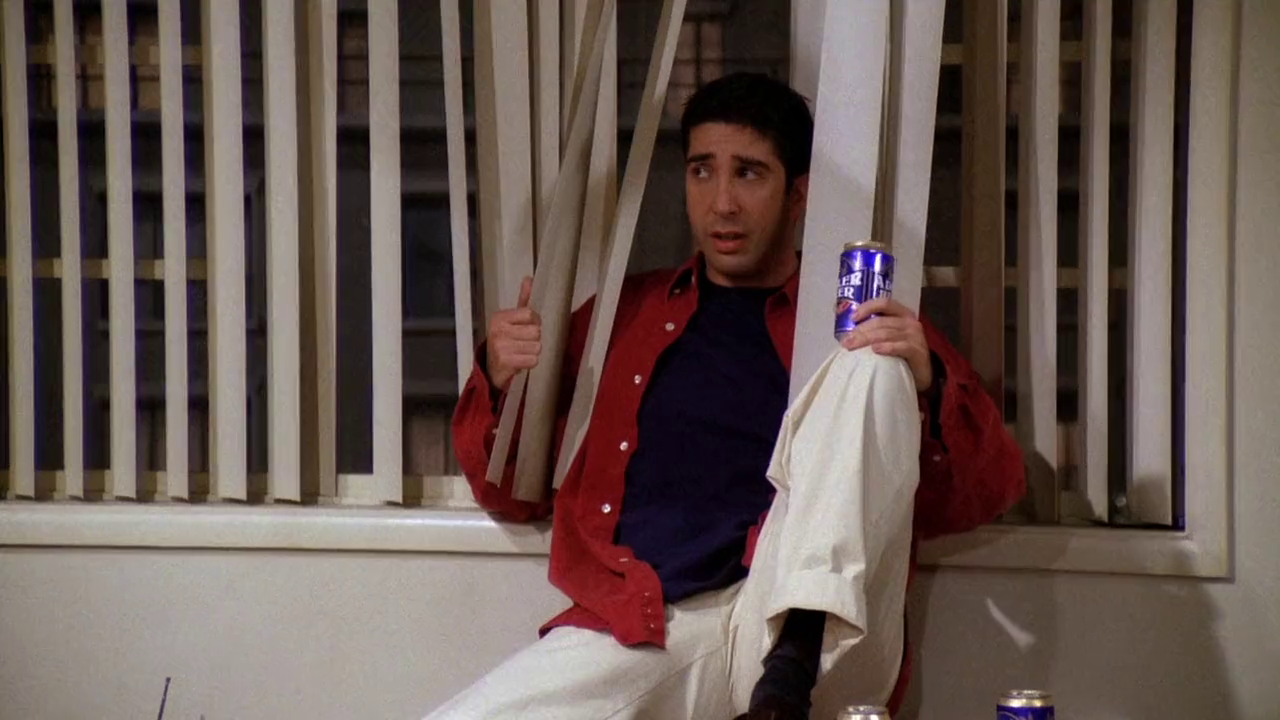
\includegraphics[trim={0 6.5cm 0 2.5cm,}, clip, width=\paperwidth]{./S01/img/1/billy-dont-be-a-hero.png}
    \caption{Billy, don’t be a hero\label{fig:billy-don-t-be-a-hero}}
  \end{adjustwidth}
\end{figure}

\begin{tcolorbox}[enhanced,center upper,
    drop fuzzy shadow southeast, boxrule=0.3pt,
    lower separated=false,
    colframe=black!30!dialogoBorder,colback=white]
\begin{minipage}[c]{0.14\linewidth}
  \raisebox{\dimexpr-\height+\ht\strutbox\relax}{
    
\includegraphics[width=1.5cm]{./assets/img/ross.png}
  }
   & \centering \scriptsize{Ross}
\end{minipage}
\hspace{.1mm}
\begin{minipage}[c]{0.8\linewidth}
  \textbf{- Do the words, 'Billy, don't be a hero', mean anything to you?}\\
  - As palavras, 'Billy, don't be a hero', significam alguma coisa pra vocês?
\end{minipage}
\end{tcolorbox}

\saveparinfos
\noindent
\begin{minipage}[c]{0.5\textwidth}\useparinfo

Ross faz menção a música \emph{Billy, don't be a hero} (1974) composta
por Mitch Murray e Peter Callander. Lançada inicialmente no Reino Unido
na voz de \emph{Paper Lace}, foi logo em seguida lançada também nos
Estados Unidos pelo grupo \emph{Bo Donaldson and The Heywoods.}

\end{minipage}\hfill
\begin{minipage}[c]{0.5\textwidth}

\begin{figure}
  \centering
  \begin{tikzpicture}
    \node [inner sep=0pt] at (0,0) {
      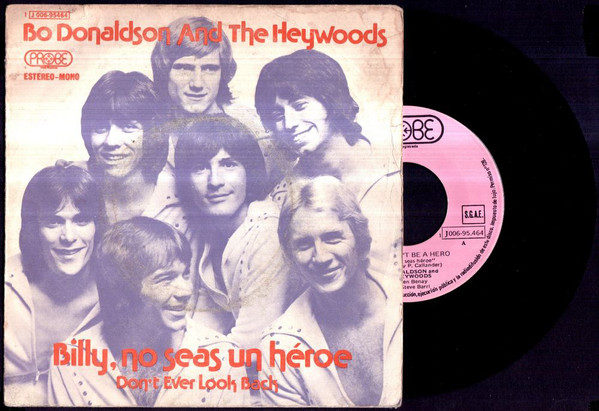
\includegraphics[width=0.8\textwidth,keepaspectratio]{./S01/img/1/billy-dont-be-a-hero-single.jpg}
    };
    \draw [white, rounded corners=\ClipSep, line width=\ClipSep]
    (current bounding box.north west) --
    (current bounding box.north east) --
    (current bounding box.south east) --
    (current bounding box.south west) -- cycle
    ;
    \end{tikzpicture}
    \caption{Billy, don’t be a hero - Single\label{fig:billy-don-t-be-a-hero-single}}
\end{figure}

\end{minipage}

\hypertarget{referuxeancias-6}{%
\subsection{Referências}\label{referuxeancias-6}}

\begin{itemize}
\tightlist
\item
  \sloppy Site Oficial. \url{http://www.bodonaldson.net/}
\item
  \sloppy IMDB. \url{https://en.wikipedia.org/wiki/Billy_Don%27t_Be_a_Hero}
\item
  \sloppy Letra - MetroLyrics. \url{https://www.metrolyrics.com/billy-dont-be-a-hero-lyrics-paper-lace.html}
\item
  \sloppy Billy, don’t be a hero - YouTube. \url{https://www.youtube.com/watch?v=1qlK9TJvuSk}
\end{itemize}

\hypertarget{pinocchio}{%
\section{Pinocchio}\label{pinocchio}}

\begin{figure}[!ht]
  \begin{adjustwidth}{-\oddsidemargin-1in}{-\rightmargin}
    \centering
    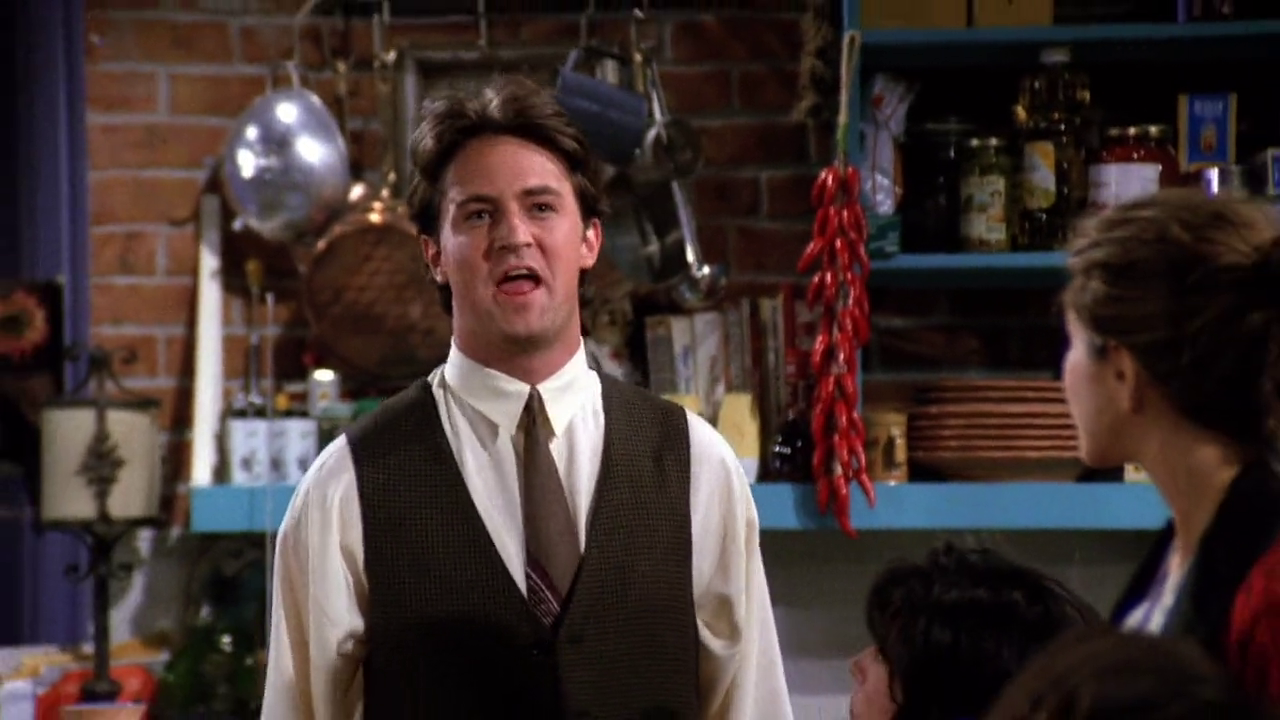
\includegraphics[trim={0 5cm 0 2cm,}, clip, width=\paperwidth]{./S01/img/1/pinocchio.png}
    \caption{Pinocchio\label{fig:pinocchio}}
  \end{adjustwidth}
\end{figure}

\begin{tcolorbox}[enhanced,center upper,
    drop fuzzy shadow southeast, boxrule=0.3pt,
    lower separated=false,
    colframe=black!30!dialogoBorder,colback=white]
\begin{minipage}[c]{0.14\linewidth}
  \raisebox{\dimexpr-\height+\ht\strutbox\relax}{
    
\includegraphics[width=1.5cm]{./assets/img/monica.png}
  }
   & \centering \scriptsize{Monica}
\end{minipage}
\hspace{.1mm}
\begin{minipage}[c]{0.8\linewidth}
  \textbf{- Wait, unless you happened to catch the Reruns' production of Pinocchio.}\\
  - Espera, a não ser que tenha visto a refilmagem do Pinóquio.
\end{minipage}

\medskip
\begin{minipage}[c]{0.14\linewidth}
  \raisebox{\dimexpr-\height+\ht\strutbox\relax}{
    
\includegraphics[width=1.5cm]{./assets/img/chandler.png}
  }
   & \centering \scriptsize{Chandler}
\end{minipage}
\hspace{.1mm}
\begin{minipage}[c]{0.8\linewidth}
  \textbf{- Look, Gepetto, I'm a real live boy.}\\
  - Olha, Gepetto, sou um menino de verdade.
\end{minipage}
\end{tcolorbox}

\saveparinfos
\noindent
\begin{minipage}[c]{0.5\textwidth}\useparinfo

Referência ao filme \emph{Pinocchio} (1940) ou \emph{Pinóquio} como
ficou conhecido no Brasil. Produzido pela \emph{Walt Disney}, o filme
conta a história de um velho carpinteiro chamado \emph{Gepetto}, que faz
um boneco de madeira chamado \emph{Pinóquio}, o qual é trazido a vida
pela \emph{Fada Azul}, com a condição de que ele demonstre obediência,
bravura e lealdade a seu criador.

\end{minipage}\hfill
\begin{minipage}[c]{0.5\textwidth}

\begin{figure}
  \centering
  \begin{tikzpicture}
    \node [inner sep=0pt] at (0,0) {
      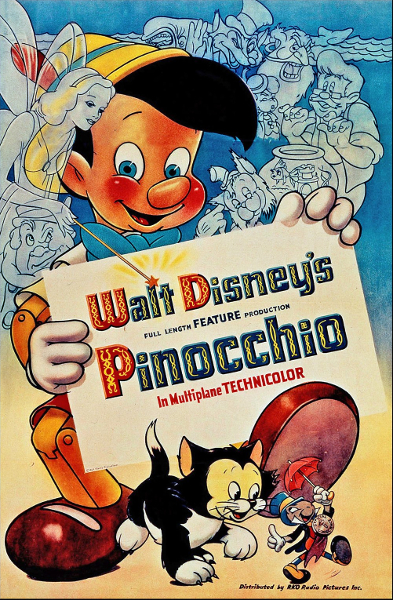
\includegraphics[width=0.5\textwidth,keepaspectratio]{./S01/img/1/pinocchio-poster.jpg}
    };
    \draw [white, rounded corners=\ClipSep, line width=\ClipSep]
    (current bounding box.north west) --
    (current bounding box.north east) --
    (current bounding box.south east) --
    (current bounding box.south west) -- cycle
    ;
    \end{tikzpicture}
    \caption{Pinocchio - Poster\label{fig:pinocchio-poster}}
\end{figure}

\end{minipage}

O filme tem muitos trechos musicais, e é daí que o Chandler retira
inspiração para a música que ele canta ao sair do apartamento:

\bigskip
\begin{tcolorbox}[enhanced,
    drop fuzzy shadow southeast, boxrule=0.3pt,
    lower separated=false, sidebyside, sidebyside align=top,
    halign=flush right, halign lower=left,
    colframe=black!30!dialogoBorder,colback=musicaBg]
\includegraphics[width=0.4cm]{./assets/img/icon-music.png}\\
Once I was a wooden boy,\\a little wooden boy…\\
\tcblower
\includegraphics[width=0.4cm]{./assets/img/icon-language.png}\\
Uma vez eu era um garoto de madeira,\\Um pequeno garoto de madeira…\\
\end{tcolorbox}

\hypertarget{referuxeancias-7}{%
\subsection{Referências}\label{referuxeancias-7}}

\begin{itemize}
\tightlist
\item
  \sloppy IMDB. \url{https://www.imdb.com/title/tt0032910/}
\item
  \sloppy Wikipédia. \url{https://pt.wikipedia.org/wiki/Pin%C3%B3quio_(filme)}
\end{itemize}

\hypertarget{liza-minnelli}{%
\section{Liza Minnelli}\label{liza-minnelli}}

\begin{figure}[!ht]
  \begin{adjustwidth}{-\oddsidemargin-1in}{-\rightmargin}
    \centering
    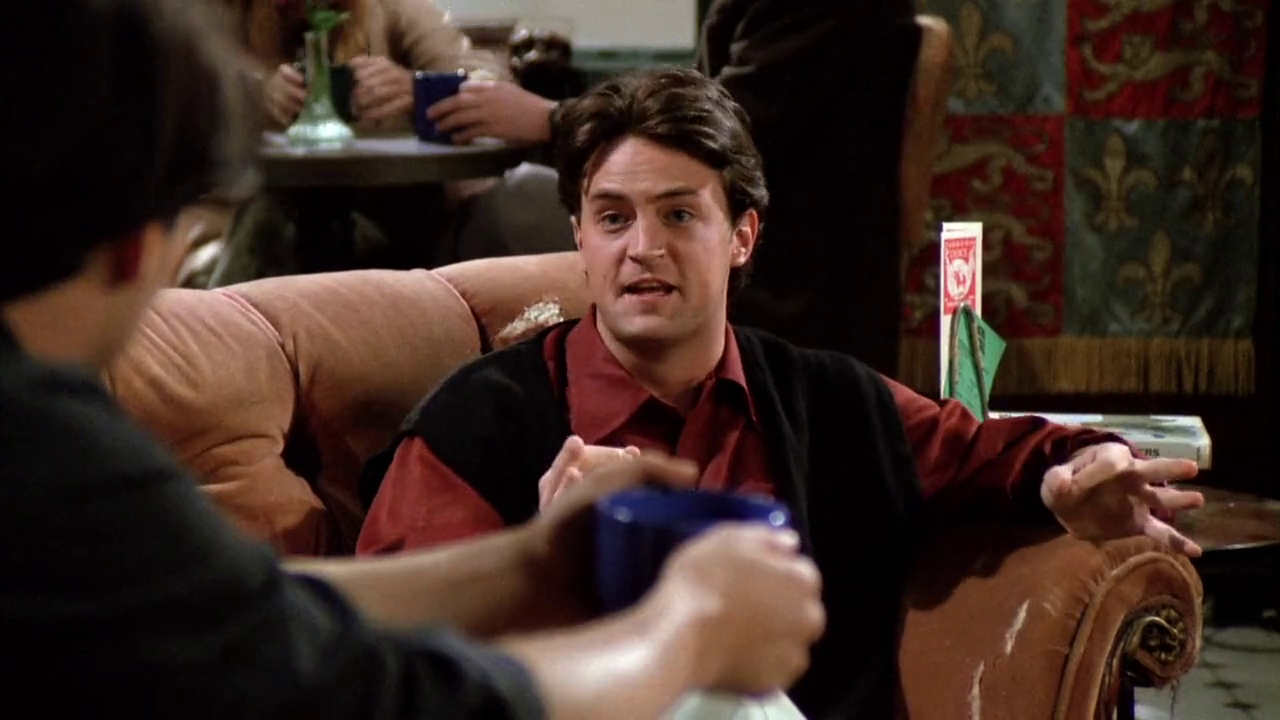
\includegraphics[trim={0 5cm 0 2cm,}, clip, width=\paperwidth]{./S01/img/1/liza-minnelli.png}
    \caption{Liza Minnelli\label{fig:liza-minnelli}}
  \end{adjustwidth}
\end{figure}

\begin{tcolorbox}[enhanced,center upper,
    drop fuzzy shadow southeast, boxrule=0.3pt,
    lower separated=false,
    colframe=black!30!dialogoBorder,colback=white]
\begin{minipage}[c]{0.14\linewidth}
  \raisebox{\dimexpr-\height+\ht\strutbox\relax}{
    
\includegraphics[width=1.5cm]{./assets/img/chandler.png}
  }
   & \centering \scriptsize{Chandler}
\end{minipage}
\hspace{.1mm}
\begin{minipage}[c]{0.8\linewidth}
  \textbf{- Kids, new dream. I'm in Las Vegas. I'm Liza Minnelli.}\\
  - Crianças, novo sonho. Tô em Las Vegas. Eu sou Liza Minelli.
\end{minipage}
\end{tcolorbox}

\saveparinfos
\noindent
\begin{minipage}[c]{0.5\textwidth}\useparinfo

Chandler menciona a atriz e cantora americana \emph{Liza Minnelli}
(1946-), é conhecida por ganhar o Oscar de melhor atriz por sua atuação
no filme \emph{Cabaret} (1972).

\end{minipage}\hfill
\begin{minipage}[c]{0.5\textwidth}

\begin{figure}
  \centering
  \begin{tikzpicture}
    \node [inner sep=0pt] at (0,0) {
      
\includegraphics[width=0.8\textwidth,keepaspectratio]{./S01/img/1/liza-minnelli-cabaret.jpg}
    };
    \draw [white, rounded corners=\ClipSep, line width=\ClipSep]
    (current bounding box.north west) --
    (current bounding box.north east) --
    (current bounding box.south east) --
    (current bounding box.south west) -- cycle
    ;
    \end{tikzpicture}
    \caption{Liza Minnelli - Cabaret\label{fig:liza-minnelli-cabaret}}
\end{figure}

\end{minipage}

\hypertarget{referuxeancias-8}{%
\subsection{Referências}\label{referuxeancias-8}}

\begin{itemize}
\tightlist
\item
  \sloppy IDMB. \url{https://www.imdb.com/name/nm0591485/}
\item
  \sloppy Wikipédia. \url{https://pt.wikipedia.org/wiki/Liza_Minnelli}
\end{itemize}
